\section{Ricorsione canonica}


\begin{frame}
  \frametitle{Funzione di partizione}
  \framesubtitle{}
  
    \centering
    Sistema ad $N$ particelle ideale
    \vspace{6pt}
    $$
        Z_N\,=\,\frac{1}{N}\sum_{k\,=\,1}^{N} z_kZ_{N-k}
    $$
    $$
        \left<E\right>\,=\,-\frac{1}{NZ_N}\sum_{k\,=\,1}^N\left(\frac{\partial z_k}{\partial \beta}Z_{N-k}\,+\,z_k\frac{\partial Z_{N-k}}{\partial \beta}\right)
    $$
    $$
        N_0\,=\,\frac{1}{Z_N}\sum_{k\,=\,1}^{N} Z_{N-k}
    $$


\end{frame}


\begin{frame}
    \frametitle{Frazione di condensato}
    \framesubtitle{}

    \begin{columns}
        \begin{column}{0.3\textwidth}
            $$
                N_0\,=\,\frac{1}{Z_N}\sum_{k\,=\,1}^{N} Z_{N-k}
            $$
        \end{column}
        
        \begin{column}{0.7\textwidth}
          \begin{figure}
              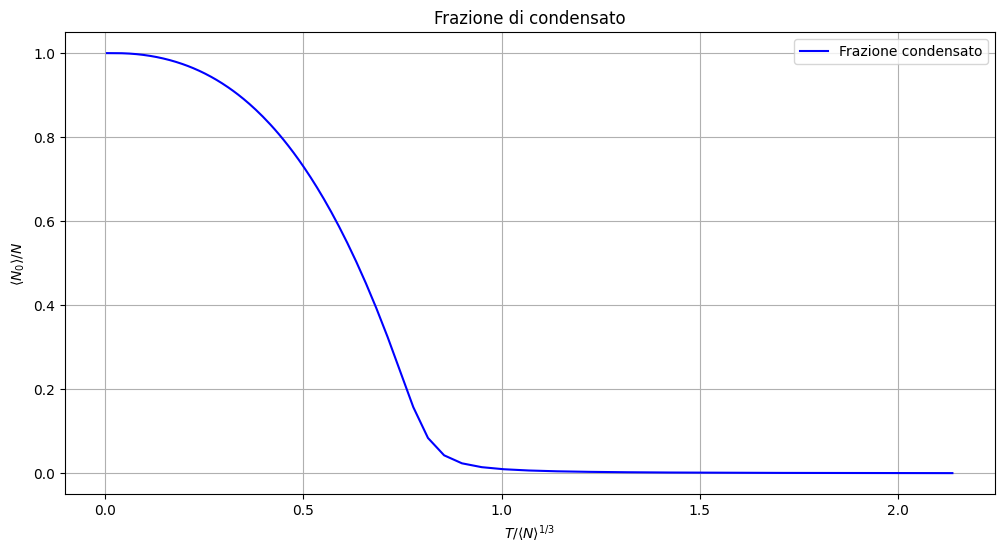
\includegraphics[width=\textwidth]{Immagini/frazCondRic.png}
              \caption{Frazione di condensato calcolata con la tecnica di ricorsione.}
          \end{figure}
        \end{column}
      \end{columns}
  
\end{frame}

\begin{frame}
    \frametitle{Calore specifico}
    \framesubtitle{}

    \begin{columns}
        \begin{column}{0.3\textwidth}
            \begin{itemize}[itemsep=0.5em, label=$\bullet$]
                \item Ritrovo il limite classico per $T \rightarrow \infty$
                \item Picco in corrispondenza del punto critico
            \end{itemize}
        \end{column}
        
        \begin{column}{0.7\textwidth}
          \begin{figure}
              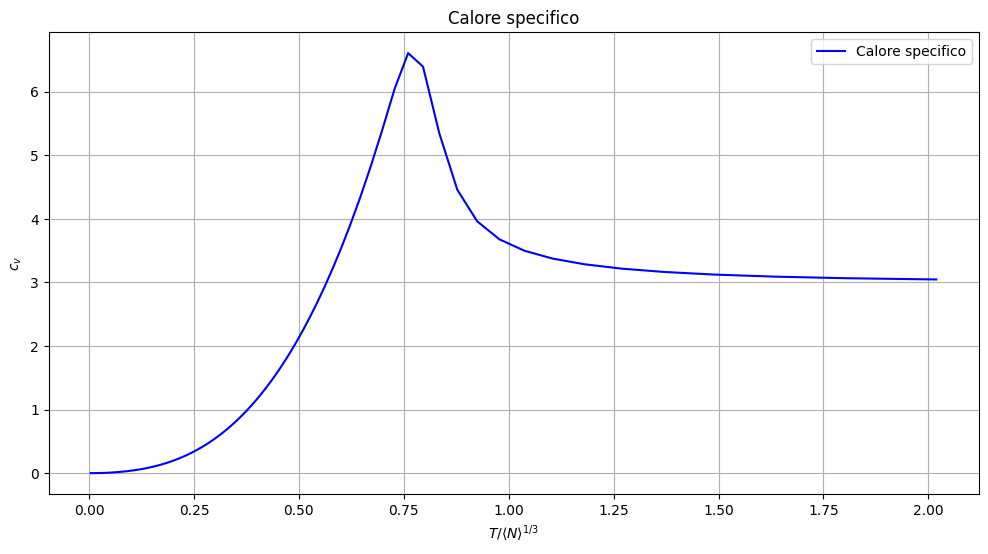
\includegraphics[width=\textwidth]{Immagini/calSpeRic.png}
              \caption{Calore specifico valutato con la tecnica ricorsiva.}
          \end{figure}
        \end{column}
      \end{columns}
  
\end{frame}
